% \section{Stereo Geometry and Emulation in VR}
% \label{sec:model}
% In this section we briefly overview stereo intersection geometry that describes the mathematical consequences of rendering and viewing errors. The principles behind this model are individually straight-forward, but the interactions become complex. A stand-alone interactive visualizer is provided in supplementary materials, and we highly encourage readers to use this tool to explore these interactions in more depth (Figure~\ref{fig:geometric_model}). We also describe our error emulation platform that we used to conduct user studies presented in Section~\ref{sec:reaching} and Section~\ref{sec:visual}. 

% \subsection{Model Overview for Interactive Simulator}
% \label{sec:model overview}
% There are lawfully-defined geometric consequences from rendering and viewing errors that can be determined using basic ray-intersection and previous works can be referenced for a  geometric derivation of the trigonometry underlying this framework \cite{held2008misperceptions, woods93, rolland04}. Rather than re-derive these equations here, we instead aim instead to give readers an intuition for how these errors arise and how they interact in our interactive application (Figure~\ref{fig:geometric_model}) in the supplementary materials. The "point" visualization mode to interactively understand how rendering errors, viewing errors, virtual image distance, and scene geometry interact.

% In a typical head-mounted display render and viewing pipeline stereo geometry errors can be introduced during rendering (Figure~\ref{fig:teaser}A or viewing (Figure~\ref{fig:teaser}B). If a viewer's eye is on-axis with an actual sphere in the world, then the corresponding image on the viewer's retina is a circle. In a typical HMD, stereo image pairs are first captured by the render cameras and shown on displays (one for each eye) to be viewed by the user. The render camera and CoP of the user's eye must coincide with the HMD CoP in order for an HMD user to perceive stereo geometry consistent with the intended 3D scene. Figure~\ref{fig:rendering_vs_viewing_error}A illustrates this process; the camera first renders a perspective projection of the sphere to a circle, this circle is shown on the display, and the user views this image and a the image of circle is formed on the retina. The rest of Figure~\ref{fig:rendering_vs_viewing_error} shows the consequences of displacements of the render cameras, user's eyes (user eye CoP), or both from the HMD CoP. We define \textit{rendering errors} as displacements of the render camera relative to the HMD CoP and \textit{viewing errors} as displacements of the user eye CoP relative to the HMD CoP. 

\section{Stereo Geometry and Emulation in VR}
\label{sec:model}
This section outlines the stereo intersection geometry governing rendering and viewing errors. While the principles behind this model are individually straightforward, their interactions are complex. We encourage readers to explore these interactions in depth using the interactive visualizer provided in the supplementary materials (Figure~\ref{fig:geometric_model}). Additionally, we describe the error emulation platform used for the user studies presented in Sections~\ref{sec:reaching} and \ref{sec:visual}.

\subsection{Model Overview}
\label{sec:model overview}
The geometric consequences of rendering and viewing errors are determined by basic ray-intersection and have been derived in previous works~\cite{held2008misperceptions, woods93, rolland04,holloway1997}. Rather than re-deriving these equations, we focus on the intuition regarding how rendering errors, viewing errors, virtual image distance (VID), and scene geometry interact. More details, and an interactive web application (Figure~\ref{fig:geometric_model}) can be found in the supplementary materials.

In a typical HMD pipeline, accurate stereo perception requires the render camera and the user's eye Center of Projection (CoP) to coincide with the HMD CoP. Deviations from this alignment can introduce errors at two stages:

\begin{enumerate}
    \item Rendering Errors: Displacements of the render camera relative to the HMD CoP (Figure~\ref{fig:teaser}A).
    \item Viewing Errors: Displacements of the user eye CoP relative to the HMD CoP (Figure~\ref{fig:teaser}B).
\end{enumerate}

Figure~\ref{fig:rendering_vs_viewing_error}A illustrates the ideal process: a sphere in the world is projected as a circle on the display, which is then projected to a circle on the user's retina. Subsequent panels in Figure~\ref{fig:rendering_vs_viewing_error} demonstrate the geometric consequences when the render cameras or user eyes are displaced from the HMD CoP. To contextualize these consequences, we next explore how misalignments between the viewer's egocentric coordinate frame and the headset's coordinate frame (e.g., via eye relief errors) can affect perceived distance.

 \begin{figure}
	     \centering
	     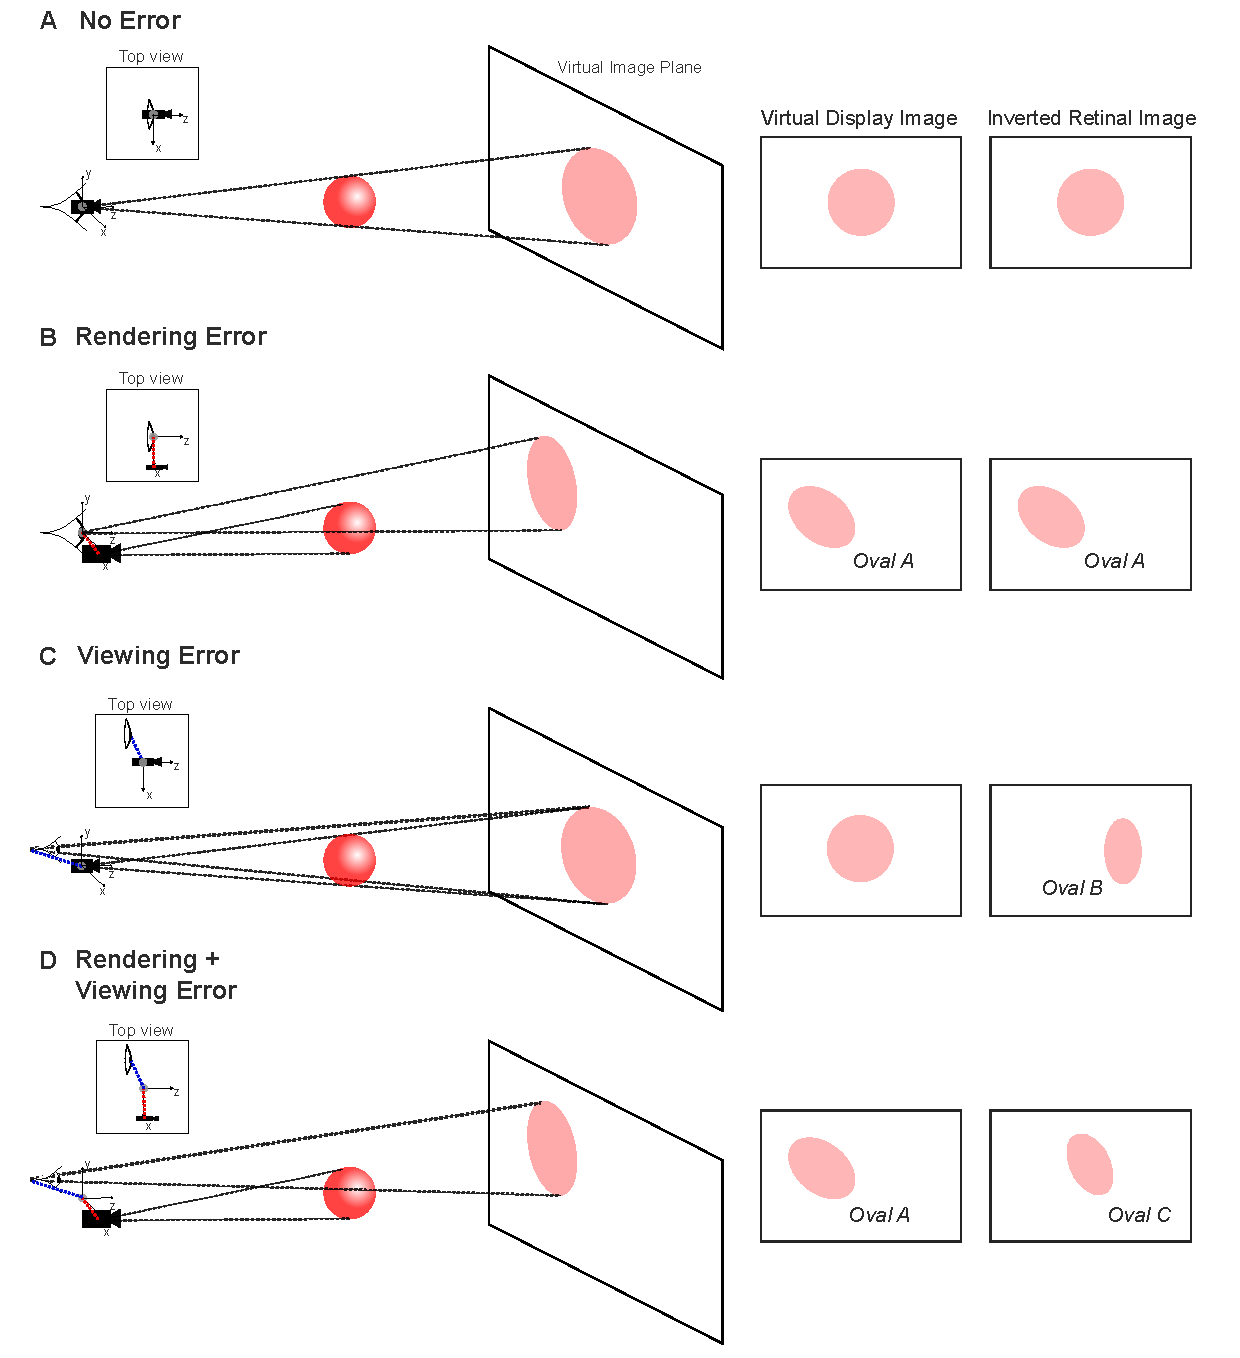
\includegraphics[width=\linewidth]{figures/model/rendering_vs_viewing_error.pdf}  
	     \caption{Comparing rendering error with viewing error. For simplicity, we show a monocular example as the set up is the same for both eyes. The origin of the coordinate system is at the HMD CoP (grey dot). The virtual sphere is positioned directly in front of the the HMD CoP. \textbf{(A)} In the ideal scenario, the render camera, CoP of the user's eye, and HMD CoP are all at the same position in space. No rendering or viewing error exists in this system. The camera is on-axis with the sphere and will render the corret perspective projection (a circle) that will be presented on virtual image plane. The user will view this circle from the intended CoP and the user's retinal image of what is shown on the display plane is also a circle. \textbf{(B)} The render camera is displaced to the right and down from the HMD CoP, creating a rendering error. The camera will render the sphere from this incorrect location, and render an oval instead of a circle. This oval is shown on the display plane and the user views it from the correct position so they perceive the same incorrectly rendered oval. \textbf{(C)} The CoP of the user's eye is displaced to the left and behind the HMD CoP, creating a viewing error. Despite the rendered image being correct on the virtual image plane, the perceived image is distorted. \textbf{(D)} In realistic usage, rendering and viewing errors typically occur together and can result in geometric errors being introduced in both render and viewing stages.}
	     \label{fig:rendering_vs_viewing_error}
	 \end{figure}


\subsection{Coordinate Systems and Distance Measurement}
Distance perception in HMDs involves two distinct coordinate systems. The origin of the \textit{HMD coordinate system} is centered between the two HMD CoPs; the intended virtual scene is defined within this frame. However, the user perceives distance relative to their own body. The \textit{egocentric coordinate system} is therefore defined relative to the viewer, with the origin centered between the user's actual left and right eye CoPs.

Ideally, these two systems align. However, viewing errors—such as eye relief shifts—introduce offsets between the egocentric and HMD frames (this is a simplified framework that does not account for the optical effects of HMD optics). This misalignment has critical implications for measuring distance perception. For example, consider a viewer with a $+3$~cm eye relief error fixating on a target at the virtual image distance (VID) (Figure~\ref{fig:error_choices}C). While the target's position is unchanged in the HMD frame, the user's eyes are physically closer to the VID. Consequently, the distance perceived in the egocentric frame is $3$~cm shorter than the distance defined in the HMD frame (Figure~\ref{fig:geometric_model}).

Crucially, standard blind reaching tasks tracked via external systems typically report positions in HMD coordinates, thereby missing this egocentric shift. To address this, Section~\ref{sec:reaching} leverages eye tracking to record reaching data that explicitly accounts for the offset between egocentric and HMD coordinates. This allows us to analyze data in either frame, distinguishing between reach accuracy (HMD frame) and accurately perceived distance (egocentric frame).


% Near-eye optics in an HMD generally have an eyebox, a volume of space from which the user should view the display for the acceptable image quality \cite{cholewiak2020}. Within the eyebox there is usually a nominally designed location where image quality is best. This location is typically selected as the display CoP typically positioned when the user's actual eye position is unknown~\cite{Rong25}. 


%In ideal circumstances an HMD will fit on a viewer's head exactly as designed and the HMD (i.e., world) coordinate frame will be exactly aligned with the user's egocentric reference frame. However, some viewing errors such as an eye relief error will shift the headset's coordinate system relative to user. When this occurs the distance perceived by the user will not directly map to the intended distance in the headset's coordinate frame. For example, consider a case where a viewer fixates on a point rendered on the optical display plane with a -3 cm eye relief error (i.e, the viewer's eyes are 3 cm farther away from the display than expected). Since the fixation target is on the display plane, the user will also perceive the point at the display plane. In HMD coordinates there is no error since the perceived point is at the intended location (i.e., on the display plane). However, in egocentric coordinates the perceived point will be 3 cm farther from the user than specified by the virtual geometry (Figure~\ref{fig:geometric_model}). 

% Consider moving these to the discussion
%The difference between perceived distance in egocentric and HMD coordinates is not simply a semantic distinction. If the viewer were perfectly accurate at estimating distance, then a verbal distance estimate would be 3 cm larger than the distance measured by an outside observer or tracking system. In other words, characterizing distance perception using verbal report and blind reaching could lead to different conclusions. In some cases, egocentric and HMD measurements can lead to opposite conclusions. In Figure~\ref{fig:geometric_model} the row of objects in front of the display closest to the viewer will appear to be too far away if measured using blind reaching, and too near if measured using verbal reports. Similarly, the middle row of objects at and near the display plane will be measured at the correct locations in HMD coordinates (i.e., with blind reaching), but will be recorded as too close in egocentric coordinates (i.e., verbal estimate). This a critical point that illustrates the importance of measuring errors using a clear, consistent framework. Notably, we can analyze reach data in both coordinate frames because we measure each participant's actual user eye position in our HMD with an eye tracker. This allows us to transform the data into the appropriate coordinate frame to evaluate absolute reach accuracy in HMD coordinates and perceived distance in egocentric coordinates.

% Here the intended target is rendered at 40 cm from the headset's original (i.e., world coordinates). If the user is asked to reach for the target object, they will reach farther than the intended target in the headset's coordinate frame. However, the user actually perceives the target object to be closer than 40 cm, and so perceived error could be categorized as either an overestimated or underestimated distance depending on the coordinate frame.

% \begin{figure}
%     \centering
%     % \includegraphics[width=1\linewidth]{figures/model/Untitled.png}
%     \includegraphics[width=1\linewidth]{figures/model/egocentric_frame.png}    
%     \caption{Placeholder.}
%     \label{fig:egocentric_frame}
% \end{figure}

% Since we show people images of the wrong thing from the right place, we don't get the same effect as if people saw the right thing from the wrong place. Need to do a simple transform to get things back into the expected world-centric cooridnate frame instead of egocentric.
% In the absence of viewing error, these two reference frames are the same, however, viewing errors always offset these two reference frames.

\subsection{HMD Error Simulation Platform} \label{sec:hmd_platform}
\paragraph{Hardware}
We integrated a 240 Hz Tobii (Tobii AB, Sweden) eye tracker into a Meta Quest 3 (v72). For each user, lens were physically adjusted to match the user's IPD. For reaching experiments in Section~\ref{sec:reaching}, we tracked controller 3D position using the default Quest API. We measured controller tracking accuracy and found that tracking is accurate within 1.5 mm error across ten distances from 5 to 50 cm, measured from the front surface of the headset (see supplementary materials). 

\paragraph{Software} 

%We build a rendering pipeline in Unity (v2022.3.30f1) that can simulate the rendering and viewing errors outlined in Section~\ref{sec:model overview}. Our application uses multiple cameras and quads for ray capture and reprojection to accomplish this, and a high-level overview is provided here. Step-by-step rendering details are provided in the supplementary materials. First a pair of render cameras render the scene and sends their framebuffers to a pair of quads simulating the virtual displays in front of HMD CoP. The VID (virtual image distance) was set to 1.3 m, approximating a reasonable VID similar to most modern HMDs designed minimize vergence-accommodation conflict~\cite{hoffman2008vergence}. Render error can be applied as a displacement of the render camera from the HMD CoP. Next, a pair of "viewing" cameras (implemented as standard camera object) view the virtual display quads from the previous step. The viewing cameras are meant to simulate user CoP in our \textit{simulated} headset space. Viewing error is applied as a displacement of the viewing camera from the HMD CoP. Lastly, the user's eyes are unlikely to be at the nominally assumed position within the Quest 3 eyebox, so we must also compensate for this naturally-occurring viewing error in the headset. This is accomplished by placing a pair of quads showing viewing camera's framebuffer in front of the actual user's 3D pupil positions from the eye tracker. These quads showing the user's expected view of the simulated rendering and/or viewing errors are imaged by the standard OVRCameras (which are positioned at actual headset CoP, not at the user's actual eye position) and this framebuffer is shown on the Quest 3 display. 

We build a rendering pipeline in Unity (v2022.3.30f1) that can simulate the rendering and viewing errors outlined in Section~\ref{sec:model overview}. The simulated headset origin is set to the midpoint of simulated HMD CoPs, positioned at (-$\frac{IAD}{2}$, 0, 0) and ($\frac{IAD}{2}$, 0, 0) for the left and right eyes, where IAD is the interaxial distance of the simulated headset. For simplicity, we first describe the rendering algorithm for one eye only (right eye). In the rendering stage, the rendering error is the displacement $\mathbf{{E}_{rendering}}$ of the rendering camera from the HMD CoP. For an arbitrary point in the scene $\mathbf{P}$, the ray vector captured by the rendering camera is: 

\begin{equation}
	\mathbf{C} = \mathbf{P} - \mathbf{{E}_{rendering}} - (\frac{IAD}{2}, 0, 0)
\end{equation}

The captured ray is then projected onto a quad positioned at the VID (virtual image distance). The VID is set to 1.3 m, approximating a reasonable VID similar to most modern HMDs designed minimize vergence-accommodation conflict~\cite{hoffman2008vergence}. The line of projection is: 

\begin{equation}
	\label{eqn: rendering_line}
	\mathbf{R} =m \mathbf{C} + (\frac{IAD}{2}, 0, 0),  m \in \mathbb{R}
\end{equation}

The projected point is intersection of the ray with the quad and found by setting $R_{y}=VID$ and solving for $m_{0}$. Substitute $m_0$ into Equation \ref{eqn: rendering_line} gives $\mathbf{R_{0}}$. This completes the rendering stage. 

For the viewing stage, the simulated eye is displaced from the HMD CoP by the viewing error vector $\mathbf{E_{viewing}}$ and views the projected point $\mathbf{R_{0}}$. The viewing ray is: 

\begin{equation}
	\mathbf{V} = \mathbf{R_{0}} - \mathbf{E_{viewing}}- (\frac{IAD}{2}, 0, 0)
\end{equation}

Lastly, we present the simulated view to the user's actual eye. The user's eye is unlikely to be at the nominally assumed position within the Quest 3 eyebox, so we must compensate for this naturally-occurring viewing error. This is accomplished by tracking the 3D pupil position using the eye tracker and presenting the simulated view on a quad based on the actual eye position. The actual HMD origin is the midpoint of Quest 3 CoPs positioned at ($-\frac{IPD}{2}$, 0, 0) and ($\frac{IPD}{2}$, 0, 0) for the left and right eyes. The tracked eye position is \textbf{E} and the line of projection is: 

\begin{equation}
	\label{eqn: rendering_line_from_actual_eye}
	\mathbf{R'} = \mathbf{E} + n \mathbf{V},   n \in \mathbb{R}
\end{equation}

The projected point is again found by setting $R'_{y}=d$, where $d$ is the fixed distance of the quad from the actual eye and solving for $n_{0}$. Substituting $n_{0}$ into Equation \ref{eqn: rendering_line_from_actual_eye} gives the intersection point $\mathbf{R'_{0}}$. The standard OVR camera positioned at the Quest 3 CoP then views the projected point $\mathbf{R'_{0}}$ and the ray is: 

\begin{equation}
	\mathbf{V'} = \mathbf{R'_{0}} - (\frac{IPD}{2}, 0, 0)
\end{equation}

The rendering algorithm for the left eye is the same as the right eye except $\frac{IAD}{2}$ and $\frac{IPD}{2}$ are replaced with $-\frac{IAD}{2}$ and $-\frac{IPD}{2}$. The percieved point in actual HMD coordinate system ${\textbf{P}}^{HMD}_{perceived}$ is given by the intersection of the left and right rays, which is found by setting them equal to each other:

\begin{equation}
	h \mathbf{V'_{left}} - (\frac{IPD}{2}, 0, 0) =l \mathbf{V'_{right}} + (\frac{IPD}{2}, 0, 0), h, l \in \mathbb{R}
\end{equation}

The solutions are: 

\begin{equation}
		l = \frac{IPD \sqrt{{v'_{left_{y}}}^2+{v'_{left_{z}}}^2}}{\vert \mathbf{V'_{left}} \times \mathbf{V'_{right}}\vert} , h = \frac{IPD \sqrt{{v'_{right_{y}}}^2+{v'_{right_{z}}}^2}}{\vert \mathbf{V'_{left}} \times \mathbf{V'_{right}}\vert} 
\end{equation}

The perceived point in egocentric coordinate system is obtained by subtracting off the translation of the interocular axis origin from the HMD origin: 

\begin{equation}
	{\textbf{P}}^{egocentric}_{perceived} = {\textbf{P}}^{HMD}_{perceived} - (0, 0, E_{eye\,relief})
\end{equation}

The experimentally measured natural eye relief error $E_{eye\,relief}$ was 13 mm on average (Table 1, supplementary materials). More information on the rendering pipeline can be found in the supplementary materials where we provide step-by-step ray tracing diagrams for illustration.

% For this we estimate actual user CoP by querying their 3D pupil positions from the eye tracker and present the frame buffers of the viewing cameras in front of the actual user CoP via another pair of quads.


%First, we estimate user CoP by querying their 3D pupil position from the eye tracker and determine the offset from the HMD CoP. This offset is applied to the OVRCamera object in Unity and is the position used for left and right HMD CoPs in Figure~\ref{fig:teaser} A. Render cameras Quads representing the left and right eye virtual displays are positioned at the VID in front of each of the HMD CoPs. Rendering error is applied as a displacement to a camera relative to the HMD CoP, and the framebuffer from the render camera is drawn to the virtual display quad. Viewing error is applied as a relative displacement between the HMD CoP and a viewing camera which images the display quad. Finally, the framebuffer from the left and right eye viewing cameras are viewed by the OVRCameras and projected onto the real HMD displays.

%\paragraph{Coordinate Frames} In our system we track user eye position and compensate for any naturally occurring viewing errors due to variations in headset fit. We then simulate and show users what they would have seen if their eyes were in a location that can be arbitrarily specified (e.g., with rendering or viewing errors). Consequently, we can show all participants the same simulated errors, regardless of where their eyes actually are. However, this means that interpreting reaching measurements from our HMD simulation platform is not always directly comparable to reach distance obtained in a headset with the actual errors being simulated.

%There are two important coordinate frames in our study: (1) HMD coordinates, and (2) egocentric coordinates. All reach data is recorded in HMD coordinates, but blind reaching data cannot be directly interpreted using these values. Since blind reaching is an open-loop task, reach distances are made in egocentric coordinates (i.e., a distance relative to the participant) so any offsets between egocentric and HMD origins must be accounted for (e.g., any eye relief errors that offset the HMD origin from the viewer's cyclopean eye). Therefore blind reach distances presented in HMD coordinates are first converted into egocentric coordinates, then converted back into HMD coordinates based on the simulated viewpoint position, rather than actual viewer position. The second transform from the viewer's actual eye position to the simulated viewpoint is important to illustrate where a participant would reach if their eyes were at the simulated location, rather than where their eyes actually are. Sighted reaching is a closed-loop task so participants must reach to the actual intended distance in HMD coordinates to generate the same stereo geometry as shown in the target interval, and egocentric conversions are unnecessary for sighted reaches. More details are provided in the supplementary materials.